
\section{Functions computed by register transducers are derivable}
\label{sec:stt-derivable}
We now  have all of the ingredients needed to derive functions computed by register transducers, as stated in the following proposition.
\begin{proposition}
    \label{prop:many-register} 
For every first-order  tree transducer, the computed function is derivable. 
\end{proposition}
The above proposition  completes the proof of the left-to-right implication in Theorem~\ref{thm:main}: we have seen, by Proposition~\ref{prop:many-register}, that first-order tree-to-tree transductions can be computed by first-order tree transducers, which are in turn derivable by Proposition~\ref{prop:many-register}.

The rest of this section is devoted to proving Proposition~\ref{prop:many-register}. To compute its output, first-order tree transducers start with relabeling the nodes of the input tree by register updates following the transition function. Since the later is a first-order tree relabeling, it is derivable thanks to Proposition~\ref{prop:forat}. To show Proposition~\ref{prop:many-register}, it remains to prove that the function
\begin{align*}
\trees(\ranked{\text{Register updates}}) \xrightarrow{\text{Evaluation}} \text{Register valuation} 
\end{align*}
which evaluates a tree of register updates to a register valuation is derivable. For that, we use  terminology inspired by universal algebra, as given in the following definition. 
\begin{definition}
    An \emph{algebra} $\alg$ consists of two sets: 
 \begin{itemize}
 \item a ranked set $\ranked{A}$ called its \emph{domain},
\item  a function $\ranked{A}\cdot A \to A$, called its \emph{shallow product}, 
 \end{itemize}
 where $A$ is the set of nullary elements of $\ranked{A}$. 
    For an algebra $\alg$, define its \emph{product} to be the function of type
    \begin{align*}
\trees( \ranked{A} ) \to A
    \end{align*}
    defined by induction on trees, using the sallow product of the algebra in the natural way.
\end{definition}
Here are some examples of algebras.
\begin{example}[The algebra of register updates] Let $\rGamma$, $\ranked{R}$ be finite ranked
sets. The \emph{algebra of register updates} over $\rGamma$, $\ranked{R}$ is the algebra whose  domain is the ranked set of register updates over output alphabet $\rGamma$ and register names $R$. The nullary elements of the domain are the register valuations.  Its shallow product is the following operation evaluating register updates 
    \begin{align*}
 {\ranked{\text{Register updates}}} \cdot {\text{Register valuations}}  \to \text{Register valuations}
    \end{align*}
The product in this algebra is the operation evaluating a tree of register updates into a register valuation. This  is the operation we are aiming to derive in this section.
\end{example}

\begin{example}[The algebra of (matrix power of) $\lambda$-terms] Let $\Tt$ be a finite set of simple types and $X$ be a finite set of typed variables. 

We define the algebra of $\lambda$-terms $\mathbf{\Lambda X}$, to be the algebra whose domain is $\ranked{\Lambda X}$, the set of $\lambda$-terms over the variables $X$ together with the error type $\ranked{\bot}$, and whose shallow product is the composition of the functions
\begin{align*}
\ranked{\Lambda X}\cdot \Lambda X \xrightarrow{\text{Flatt}} \Lambda X \xrightarrow{\text{Normal form}} \Lambda X 
\end{align*}
where Normal form is the function computing normal form of affine terms using types in $\Tt$ for their sub-terms, and associating $\bot$ to the other terms. 



Now let $k$ be an integer. We set $\mathbf{(\Lambda X)^{[k]}}$ to be the algebra whose domain is the matrix power $\ranked{\mati k {(\Lambda X)}}$, and whose shallow product is the composition of shallow unfold with the lifting of the shallow product of the algebra $\mathbf{\Lambda X}$
\begin{align*}
\ranked{(\Lambda X)^{[k]}}\cdot (\Lambda X)^{[k]} \to (\ranked{\Lambda X}\cdot \Lambda X)^{[k]}  \to (\Lambda X)^{[k]} 
\end{align*}

Thanks to Theorem~\ref{thm:normalise} and ~\ref{thm:stt}, the product of $\mathbf{(\Lambda X)^{[k]}}$ is derivable, as the composition of the following derivable functions
\begin{align*}
\trees(\ranked{\Lambda X})^{[k]} \xrightarrow{\text{Unfold}} (\trees \ranked{\Lambda X})^{[k]} \xrightarrow{\text{flatt}^{[k]}} 
 (\Lambda X)^{[k]} \underset{\text{form}}{\xrightarrow{\text{Normal}}}  (\Lambda X)^{[k]}
\end{align*}
\end{example}

To show that an algebra has a derivable product, we will be to embed it into another algebra whose 
product is known to be derivable. This justifies the following definition.

Let $\mathbf{A}$, $\mathbf{B}$ be two algebras. An \emph{embedding} of $\mathbf{A}$ into $\mathbf{B}$ is a function $\ranked{f: \ranked{A}\to \ranked{B}}$ which makes the following diagram commutes ($f$ is the restriction of $\ranked{f}$ to $A$.)
      \begin{align*}
    \xymatrix@C=2cm{
        \ranked{A} \cdot A \ar[r]^{\ranked{f}\cdot f} \ar[d]_{\text{Shallow product}} & \ranked{B}\cdot B \ar[d]^{\text{Shallow product}}\\
A \ar[r]_{f} & B       
       }
    \end{align*} 
It is easy to check that the following diagram also commutes for embeddings    
        \begin{align*}
    \xymatrix@C=2cm{
        \trees(\ranked{A}) \ar[r]^{\trees(\ranked{f})} \ar[d]_{\text{Product}} & \trees(\ranked{B}) \ar[d]^{\text{Product}}\\
A \ar[r]_{f} & B       
       }
    \end{align*}  
 In the light of this property, to show that the product of an algebra $\mathbf{A}$ is derivable, it is enough to find an algebra $\mathbf{B}$ and an embedding $\ranked{f}$ of $\mathbf{A}$ into $\mathbf{B}$ such that:  
the product of $\mathbf{B}$ is derivable, $f$ is derivable, $f$ is invertible and its inverse $f^{-1}$ is derivable.  

In our case, we will embed the algebra of register updates into an algebra $\mathbf{(\Lambda X)^{[k]}}$, for a well chosen set of variables $X$ and set of types $\Tt$. As noticed earlier, the product of the latter is derivable, we only need to show that the additional derivability conditions on the embedding.



\newpage
As said earlier, the main idea will be to relate the computation of an STT with normalization of a certain $\lambda$-term. For that, we will show in subsection~\ref{subsec:ru-as-lambda} how to encode register updates as (matrix power of) $\lambda$-terms. The proof of Proposition~\ref{prop:many-register} is then given in subsection~\ref{subsec:proof}. In the rest of this section, we suppose without loss of generality\footnote{To show that unary registers are sufficent, we can proceed by induction on the maximal arity of registers. The main observation is  that the content of a register can be split in three parts...}, that the registers of our STT are at most unary. We suppose that the input and output vocabularies of our STT are $\rSigma$ and $\rGamma$ respectively. 

\subsection{Register updates as $\lambda$-terms}\label{subsec:ru-as-lambda}
\paragraph{Terms as $\lambda$-terms.} On va d'abord commencer par rappeler un encodage assez classique des terms en $\lambda$-termes.
Les termes en general sont des objets statiques qui m'on t pas de conte nu calculatoire, c'est normal qu'ils soient représentés par des lambda termes 
\paragraph{One register.} Suppose that our STT have only one register $r$. We define the function
\begin{center}
\begin{tabular}{>{\centering\arraybackslash}m{.15\textwidth} >{\centering\arraybackslash}m{.03\textwidth} >{\centering\arraybackslash}m{.3\textwidth}}
$\ranked{\text{Register updates}}$ & $\xrightarrow{\ranked{\lambda}}$ & $\ranked{\tmonad(\set{x}^\ranked{\lambda}\ranked{+ \Gamma})}$ \\
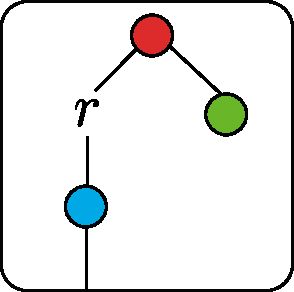
\includegraphics[scale=.3]{unary-register-update.pdf} & $\mapsto$ & 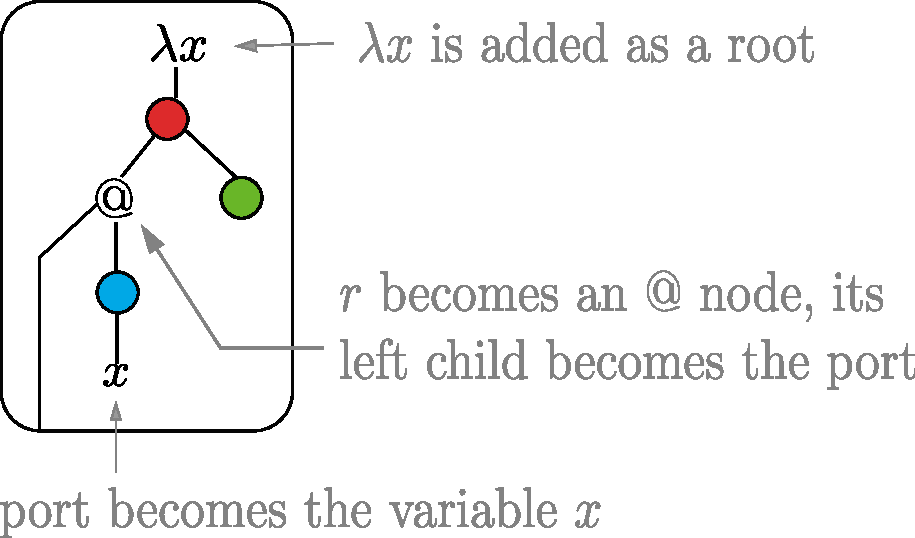
\includegraphics[scale=.3]{its-encoding.pdf}
\end{tabular}
\end{center}
The function $\lambda$ represents unary register updates (which are just terms over $\ranked{\tmonad(\Gamma+\set{r})}$) as terms over $\tmonad({x}^\ranked{\lambda}\ranked{+ \Gamma})$, where $x$ is a variable of type $o$.
 \begin{center}
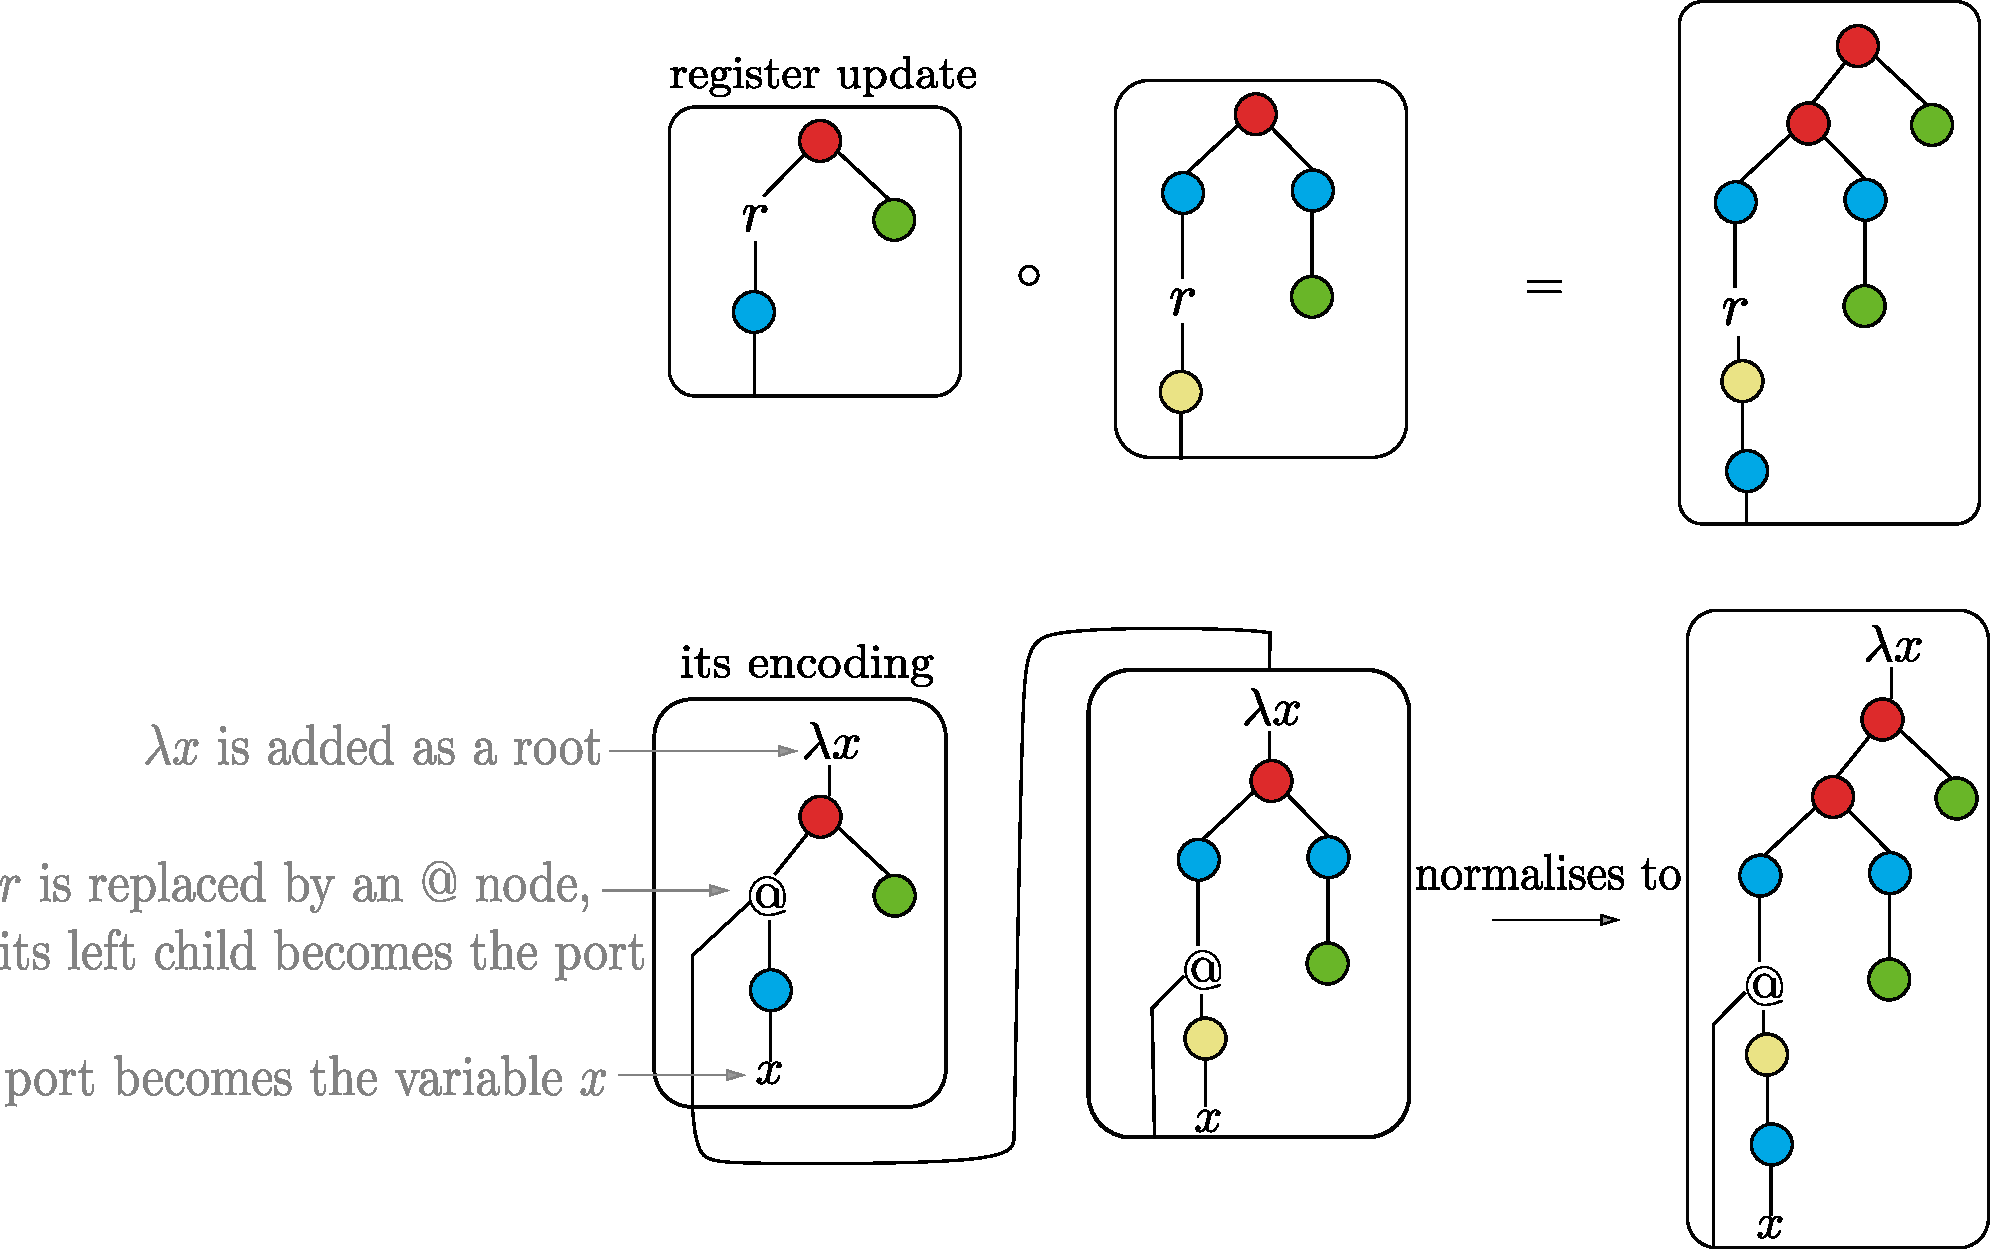
\includegraphics[scale=.26]{composition=normalisation.pdf}
\end{center}
The picture also justifies this encoding: it shows that that composition is the same thing as normalisation.

\paragraph{The general case.}

\subsection{Proof of proposition~\ref{prop:many-register}}\label{subsec:proof}

There will be four main ingredients, namely derivability for: first-order tree relabelings (Proposition~\ref{prop:forat}), normalisation of affine $\lambda$-terms (Theorem~\ref{thm:normalise}), and unfolding of the matrix power (Proposition~\ref{prop:monotone-unfold}).
\label{sec:proof-of-prop} 
To put these ingredients together,  we use  terminology inspired by universal algebra, as given in the following definition. 

\begin{definition}
    An \emph{algebra} $\alg$ consists of two sets 
    \begin{align*}
    \overbrace{\algdom \alg}^{\text{unranked}} \qquad \overbrace{\algops \alg}^{\text{ranked}},
    \end{align*}
equipped with a  \emph{shallow product}\footnote{
    A more standard approach would be to use a family of operations indexed by the signature
    \begin{align*}
    \set{f^\alg : (\algdom \alg)^{\arity f} \to \algdom \alg}_{f \in \algops \alg}.
    \end{align*}
   Our approach is equivalent, i.e.~defining a shallow product is the same as defining a family of operations.
}, which is function of type
\begin{align*}
 \shallowterm {(\algops \alg)}{\underbrace{(\algdom \alg)}_{\substack{\text{viewed as a ranked}\\ \text{set, with all elements}\\ \text{having arity zero}}}} \rto \redpar {\algdom \alg}.
\end{align*}
    For an algebra $\alg$, define its \emph{product} to be the function of type
    \begin{align*}
        \treepar {\algops \alg} \to \algdom \alg
    \end{align*}
    defined in the natural way.
    %  An algebra is called \emph{derivable} if its product  is derivable. 
\end{definition}


One example of an algebra is when the signature is some ranked set $\rSigma$, the domain is  $\trees \rSigma$, and the interpretation is defined in the natural way. In this case, the product operation is the identity. A variant of this algebra is when the signature is replaced by $\tmonad \rSigma$; in this case the product operation becomes flattening. 

Let us begin the proof of Proposition~\ref{prop:many-register}.
Fix a register transducer with $k$ registers. For the rest of this section, when talking about register valuations and register updates, we mean the registers of the fixed register transducer.
Another example of an algebra was implicit in the definition of register transducers: the domain is the register valuations and the signature is the  register updates. To prove  Proposition~\ref{prop:many-register}, we will show that the algebra of register updates embeds -- via the matrix power -- in an algebra, call it $\alg$, whose product operation is derivable as a special case of normalisation of affine $\lambda$-terms. 
 The idea behind the algebra  $\alg$ is to use  $\lambda$-terms to represent register contents, according to the following picture:
 \begin{center}
 \includegraphics[scale=.3, page=59]{pics.pdf}
 \end{center}
%    \mypic{59}  
    Let  $\nmax$  be the maximal arity of registers in the fixed register transducer, and let  $\rGamma$ be its  output alphabet. For a term $t \in \tmonad \rGamma$ of arity at most $\nmax$, its representation as a  $\lambda$-term, which we denote by $t^\lambda$,  uses variables from the following finite set (we use the notation $\otype^i \to \otype$ defined in Example~\ref{ex:affine-not-enough}):
\begin{align*}
X  \quad \eqdef \quad \set{\typevar {x_a} {\otype^i \to \otype} : a \in \rGamma \text{ of arity $i$}} \cup \set{\typevar {x_i} \otype : i \in \set{1,2,\ldots,\nmax }}.
\end{align*}
Furthermore, $t^\lambda$ is affine and it can be typed using simple types  from  the following set finite set :
\begin{align*}
    \Tt \quad \eqdef \quad \set{\otype^i \to \otype : i \in \set{0,\ldots,\nmax}}
\end{align*}
This means that if $t$ has arity at most $\nmax$ -- which is true for any term that can appear in a register of our fixed register transducer -- then its $\lambda$-term representation $t^\lambda$ satisfies constraints as in Theorem~\ref{thm:normalise}.  On its own, $t^\lambda$ is already in normal form, so there is no need to normalise it, but we intend to compose  such $\lambda$-terms, leading to terms that are not in normal form (but which still use variables from $X$ and types from $\Tt$). 
This motivates the  following definition of an algebra, call it $\alg$. Its domain and signature are given by 
\begin{align*}
\overbrace{\set \bot + \trees \lamrank X}^{\algdom \alg}  \qquad \overbrace{ \tmonad \lamrank X}^{\algops \alg} 
\end{align*}
\begin{align*}
\text{where }\lamrank X = {\overbrace{\set{x : x \in X}}^{\text{arity 0}} \cup \overbrace{\set{\lambda x : x \in X}}^{\text{arity 1}} \cup  \overbrace{\set @}^{\text{arity 2}}}
\end{align*}
In other words, the domain is $\lambda$-terms plus an error element, and the signature is $\lambda$-terms  with ports. The   product operation is 
\begin{align*}
t^\alg(t_1,\ldots,t_n) = \begin{cases}
    \text{normal form of $t(t_1,\ldots,t_n)$} & \text{if $t(t_1,\ldots,t_n)$ is affine and can be typed using $\Tt$}\\
    \bot & \text{otherwise}
\end{cases}
\end{align*}
In particular, if one of the inputs $t_1,\ldots,t_n$ is $\bot$, then the output is also $\bot$.  The algebra $\alg$ is designed so that we can apply Theorem~\ref{thm:normalise} about normalising $\lambda$-terms to see that the  product operation in the  algebra $\alg$ is derivable. Next, by observing that the matrix power is a form of syntactic sugar for manipulating registers in a register automaton, we see that there is an arity preserving 
    \begin{align*}
    \ranked h : \regups \to \mati k {(\algops \alg)}
    \end{align*}
    which has only monotone elements in its image, and which makes the following diagram commute


Putting this all together, we see that there is a derivable function which inputs a tree of register updates, and outputs the value of the first register, represented as a $\lambda$-term. The last remaining observation is that function $t^\lambda \mapsto t$, i.e.~the inverse of the $\lambda$-term representation, is derivable. This inverse can be achieved, for example, by composing a first-order tree relabelling with a tree homomorphism. This completes the proof of Proposition~\ref{prop:many-register}, and therefore also of Theorem~\ref{thm:main}. 